%===================================== CHAP 4 =================================

\chapter{Platform (?)}

In 2016, the long anticipated new hardware was finally installed and was ready
to be used for the CARP project. The new machine contains four Convey Wolverine
Application Accelerators, coprocessors aimed at accelerating key parts of
algorithms in high-performance computing through reconfigurable hardware. Each
accelerator is equipped with a state-of-the-art Xilinx FPGA and large,
high-bandwidth on-chip memory.

The following sections describe the Wolverine accelerator architecture, the
toolchain used to synthesize the hardware design and finally the toolchain used
for the software API.

\section{Convey Wolverine WX-2000 Application Accelerator}

The Convey Wolverine WX-2000 is a PCIe-mounted coprocessor equipped with a
Xilinx Virtex-7 XC7V2000T FPGA and four SO-DIMM slots allowing for up to 64 GB
of on-chip memory. \figurename~\ref{fig:convey-wx-card} shows how a Wolverine
coprocessor is organized at a high level. The host computer communicates with
the card over PCIe at a max bandwidth of 8 GB/s. On the coprocessor the Host
Interface controller (HIX) is responsible for decoding the data sent from the
host. Data can either be stored in the on-board memory, or passed directly to an
the FPGA.

With 2 million logic cells, 46 MB of BRAM and up to 2.8 Tb/s serial bandwidth,
the XC7V2000T is one of Xilinx' higher end FPGAs. Earlier, FPGAs have been
scaled monolithically following Moore's Law \todo{reference}, in the same way
conventional processors have been scaled. With the XC7V2000T however, Xilinx has
opted to combine 4 separate dies into one large virtual FPGA with their Stacked
Silicon Interconnect (SSI) technology \cite{Saban2011}. Each die, or Super Logic
Region (SLR), has its own clocking and configuration circuitry. For monolithic
designs, these signals would have to be routed throughout the entire die in
complex ways to avoid critical paths that are too long. With this circuitry
replicated in each SLR, the resources required for routing clocking and
configuration signals is significantly lower, opening up the possibility to use
these resources to interconnect the SLRs instead. This, along with advances in
manifacturing techniques has allowed Xilinx to scale their FPGAs even further
and opening up new use cases for them. Programming FPGAs using SSI is no
different from any other FPGA, the Xilinx design flow toolchain distributes
designs across multiple SLRs if needed.


\begin{figure}[ht]
  \centering
  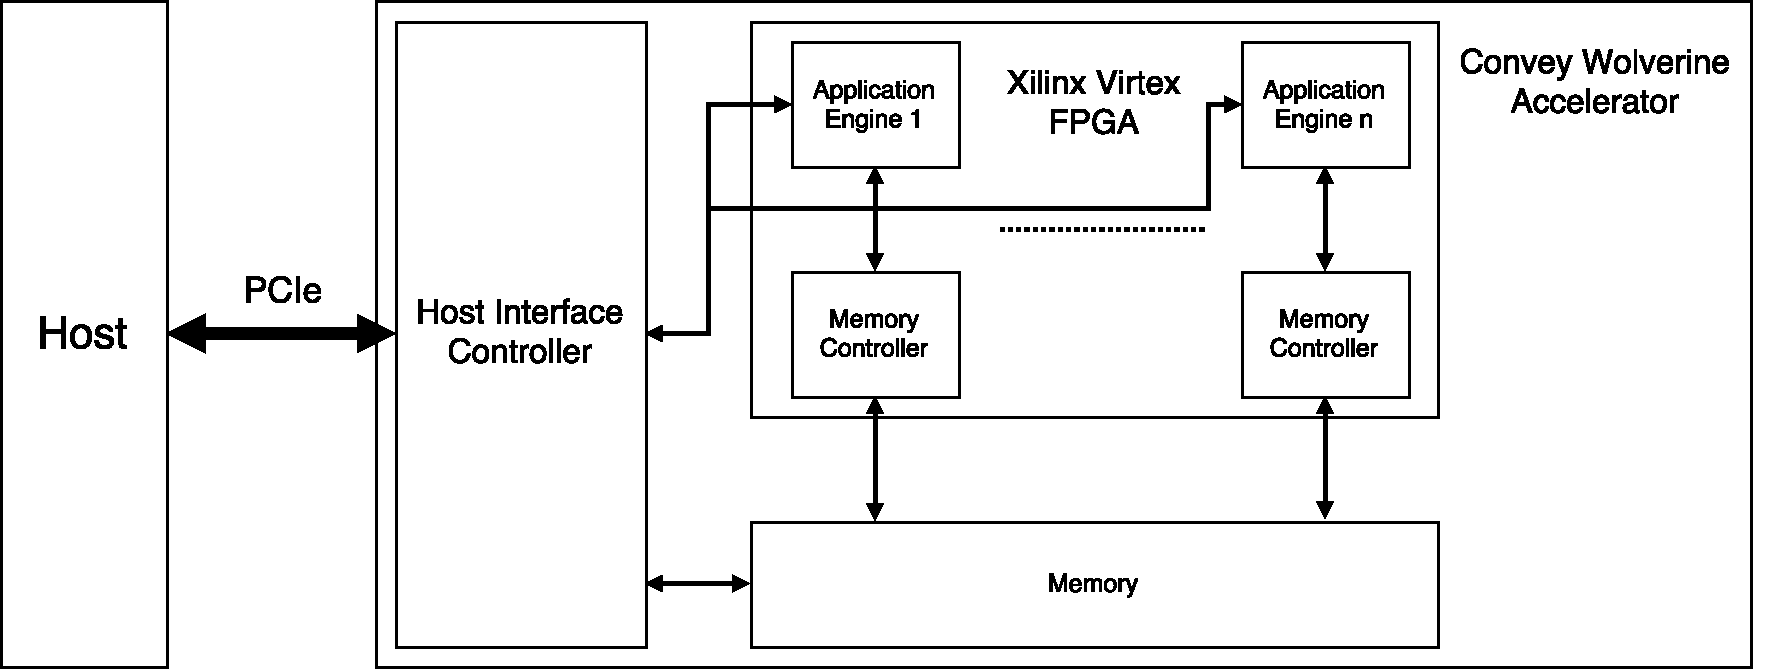
\includegraphics[width=\linewidth]{fig/convey-wx-card}
  \caption{
    High level overview of the Convey Wolverine Accelerator architecture.
    \label{fig:convey-wx-card}
  }
\end{figure}


\section{Hardware Toolchain}

All previous iterations of the CARP hardware platform have been implemented
entirely in VHDL. At the start of this project, the decision was made to start
porting the codebase to Chisel, a hardware construction DSL implemented in the
Scala programming language.

\subsection{Chisel}

Chisel\footnote{\url{https://chisel.eecs.berkeley.edu/}} is an open-source
hardware construction language developed at UC Berkeley. Where many other
hardware design tools implemented in high-level programming languages are of the
``C-to-gates'' variety, tools that try to automagically infer hardware based on
a description of the desired computation, Chisel is based upon using the
computational tools in Scala to describe how a circuit should be wired.
Leveraging Scalas typesystem and functional programming tools, Chisel encourages
code reuse, genericity and designing systems that are highly parameterizable.

Listing \ref{lst:chisel-sample} shows how to implement the circuit in
\figurename~\ref{fig:chisel-sample}. The \texttt{io} bundle defines the inputs
and outputs of the module. In this case a boolean input signal and three
unsigned integer signals, two inputs and an output, all of whose bitwidth is
determined by the \texttt{w} parameter passed to the module when it is
instantiated, i.e. \mintinline{scala}|val s = Module(new Sample(32))| will
create an instance of the \texttt{Sample} module with 32-bit wide
\texttt{UInt}s.

When executed, a Chisel program creates a internal graph representation of the
circuit described by the program. Depending on the parameters given to the
program, the program will output either Verilog or a C++ simulator of the
circuit. To create a fully functional FPGA-image the Verilog output can be
incorporated into an FPGA design flow.

To avoid having to start entirely from scratch, it was decided that porting the
CARP hardware platform to Chisel would be done in a top-down fashion. That is,
start by instantiating Lundals toplevel module as a blackbox in the Chisel
design and implement downward in the module hierarchy as needed when extending
the functionality of the platform. \figurename~\ref{fig:hw-build-process} gives
an overview of the build process. All parameterization is gathered in the Chisel
part of the design and passed on into the VHDL modules when they are
instantiated in the resulting Verilog.

For further details regarding the development setup for the hardware part of the
CARP project, see Appendix \todo{link here to readme}.

\begin{figure}
\begin{mintedsubfloat}[Chisel source \label{lst:chisel-sample}]{0.5\linewidth}
\begin{minted}[fontsize=\footnotesize]{scala}
import chisel._

class Sample(w: Int) extends Module {
  val io = new Bundle {
    val a  = UInt(INPUT, width=w)
    val b  = UInt(INPUT, width=w)
    val sel = Bool(INPUT)
    val out = UInt(OUTPUT, width=w)
  }
  val stored = Reg(init=UInt(0))
  val sum = io.a + io.b

  when (sel) {
    io.out := stored
  }.otherwise {
    stored := sum
    io.out := sum
  }
} 
\end{minted} 
\end{mintedsubfloat}
\subfloat[Circuit \label{fig:chisel-sample}]{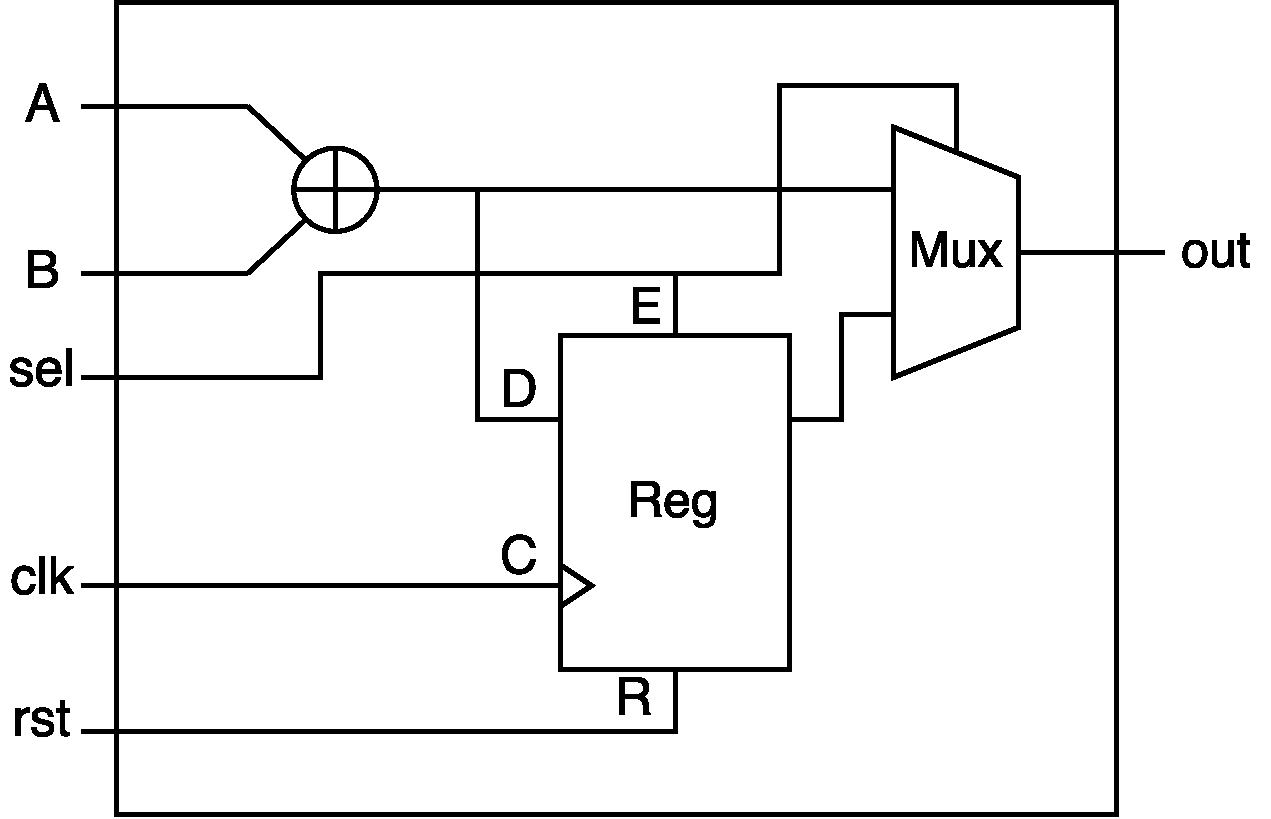
\includegraphics[width=0.5\linewidth, valign=c]{fig/chisel-sample}}
\end{figure}

\begin{figure}[ht]
  \centering
  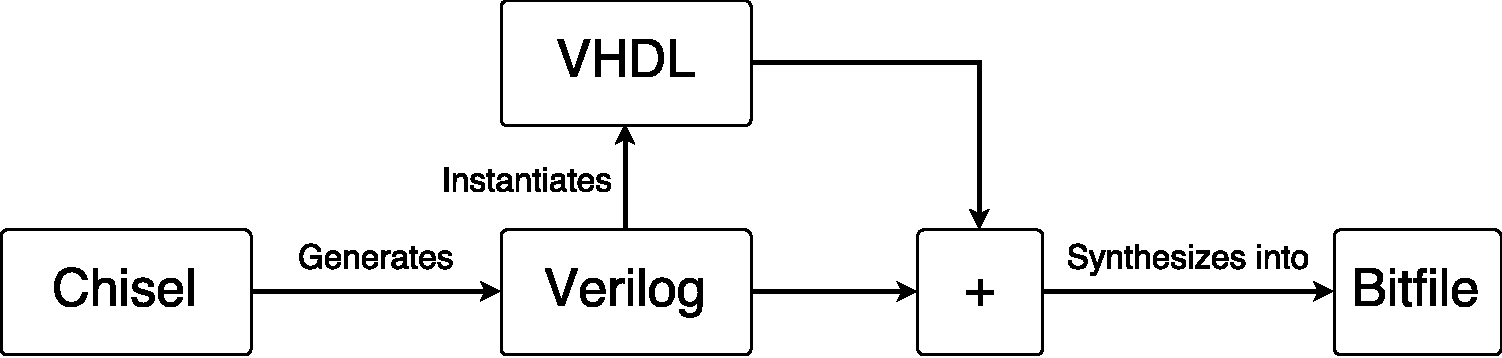
\includegraphics[width=0.8\linewidth]{fig/hardware-build-process}
  \caption{Build process overview.\label{fig:hw-build-process} }
\end{figure}

\section{Software Toolchain}

The software API is written in C, compiled on CentOS 6.5, Linux kernel version
2.6.32-431 with GCC version 4.4.7. Outside of the C standard library, the API
has only one dependency; the Convey Personality Development Kit. It is included
routines related to communicating with the Convey coprocessor.


\cleardoublepage
%%% Local Variables:
%%% mode: latex
%%% TeX-master: "../thesis"
%%% End:
